\chapter{Rheon}
\label{chap:rheon}

To evaluate whether a detector detects a drift, we need event logs with known drifts. Public event logs with known drifts are hard to find and mostly contain drifts in the control-flow perspective or timing attributes. The Concept Drift Log Generator (CDLG) developed by \textcite{grimm2022cdlg} generates synthetic event logs with control-flow drifts and the authors mention multi-perspective drifts as future work.

We introduce Rheon in this chapter in order to fill this gap. Rheon is a Python library developed in this thesis that generates synthetic event logs with injected concept drifts. It allows users to configure the generation parameters comprehensively and to inject concept drifts from intra-case, resource and inter-case perspectives. The input comprises parameters of a base process model and a list of drifts. The output is an event log with activities, timestamps, resources, two case attributes and a metadata file that comprehensively describes the base process parameters as well as the injected drifts together with their drift types. Rheon supports nine drift types from the three perspectives and the two drift modes sudden and gradual. We will use Rheon logs in Chapter~\ref{chap:eval} to evaluate our state-based framework on known drifts.

Section~\ref{sec:rheon:schema} introduces the log schema of Rheon-generated logs and gives an example. Section~\ref{sec:rheon:generation} gives an overview of the generation of an event log using Rheon. Section~\ref{sec:rheon:drifts} introduces the nine drift types supported by Rheon. In Section~\ref{sec:rheon:examples} we give examples of generated logs and figures showing the drifts visually. Section~\ref{sec:rheon:limitations} discusses the limitations and future work of Rheon.


\section{Generated Log Schema}
\label{sec:rheon:schema}
Rheon generates and writes an event log according to Definition~\ref{def:prelim:event_log} as a file in the format eXtensible Event Stream (XES) or Comma-Separated Values (CSV). Table~\ref{tab:rheon:schema} shows the nine columns of the event log schema. Amount and region are the case attributes. Rheon sorts the events according to case identifiers and start timestamps. The first event of a case starts at the arrival time of the case. All other events start after the end of the previous event and a waiting time. For all generated event logs, Rheon also creates a metadata file that includes the generation parameters and the drifts of the log. Table~\ref{tab:rheon:excerpt} provides an example of a Rheon-generated log.

\begin{table}[tb]
	\centering
	\caption[Schema of a Rheon log]{%
		The columns of a Rheon log. The level states whether an attribute belongs to an event or to a case. The column Name gives the attribute name in Definition~\ref{def:prelim:event_log}.}
	\label{tab:rheon:schema}
	\begin{tabular}{@{}lll>{\raggedright\arraybackslash}p{6.1cm}@{}}
		\toprule
		Column                       & Level &      Name                &           Meaning                                                 \\
		\midrule
		\texttt{event:id}            & event & --                  & event identifier      \\
		\texttt{case:concept:name}   & case  & $\mathit{case}$     & case identifier        \\
		\texttt{concept:name}        & event & $\mathit{act}$      & activity              \\
		\texttt{start\_timestamp}    & event & --                  & start of processing                                     \\
		\texttt{time:timestamp}      & event & $\mathit{time}$     & completion of processing                                \\
		\texttt{event:duration\_min} & event & $\mathit{duration}$ & processing time        \\
		\texttt{org:resource}        & event & $\mathit{res}$      & assigned resource   \\
		\texttt{case:amount}         & case  & $\mathit{amount}$   & case amount \\
		\texttt{case:region}         & case  & $\mathit{region}$   & case region         \\
		\bottomrule
	\end{tabular}
\end{table}

\begin{table}[tb]
	\centering
	\caption[Excerpt of a Rheon log]{%
		The first six rows of the example log with a control-flow drift from Section~\ref{sec:rheon:examples}. Identifiers are abbreviated, and timestamps are shown without year and seconds.}
	\label{tab:rheon:excerpt}
	\small
	\setlength{\tabcolsep}{2pt}
	\begin{tabular}{@{}lllllrlrl@{}}
		\toprule
		\shortstack[l]{\texttt{event:}\\\texttt{id}} & \shortstack[l]{\texttt{case:}\\\texttt{concept:}\\\texttt{name}} & \shortstack[l]{\texttt{concept:}\\\texttt{name}} & \shortstack[l]{\texttt{start\_}\\\texttt{timestamp}} & \shortstack[l]{\texttt{time:}\\\texttt{timestamp}} & \shortstack[l]{\texttt{event:}\\\texttt{duration\_}\\\texttt{min}} & \shortstack[l]{\texttt{org:}\\\texttt{resource}} & \shortstack[l]{\texttt{case:}\\\texttt{amount}} & \shortstack[l]{\texttt{case:}\\\texttt{region}} \\
		\midrule
		\texttt{evt\_1} & \texttt{case\_1} & \texttt{a} & Jan 1, 00:00 & Jan 1, 00:24 & 24.20 & \texttt{res\_03} & 1,151.36 & \texttt{region\_3} \\
		\texttt{evt\_2} & \texttt{case\_1} & \texttt{b} & Jan 1, 00:41 & Jan 1, 01:10 & 29.48 & \texttt{res\_01} & 1,151.36 & \texttt{region\_3} \\
		\texttt{evt\_3} & \texttt{case\_1} & \texttt{c} & Jan 1, 01:48 & Jan 1, 02:08 & 20.33 & \texttt{res\_01} & 1,151.36 & \texttt{region\_3} \\
		\texttt{evt\_4} & \texttt{case\_1} & \texttt{d} & Jan 1, 02:21 & Jan 1, 02:37 & 16.27 & \texttt{res\_04} & 1,151.36 & \texttt{region\_3} \\
		\texttt{evt\_5} & \texttt{case\_1} & \texttt{e} & Jan 1, 02:38 & Jan 1, 02:59 & 21.57 & \texttt{res\_01} & 1,151.36 & \texttt{region\_3} \\
		\texttt{evt\_6} & \texttt{case\_2} & \texttt{a} & Jan 1, 09:00 & Jan 1, 09:03 & 3.10  & \texttt{res\_03} & 768.65   & \texttt{region\_3} \\
		\bottomrule
	\end{tabular}
\end{table}

\section{Generation of an Event Log}
\label{sec:rheon:generation}

Similar to CDLG (\textcite{grimm2022cdlg}), Rheon describes the control-flow through a process tree (Section~\ref{sec:prelim:process_trees}) and generates traces with a play-out from a process tree.
For the generation and the play-out, Rheon uses the library PM4Py (\textcite{berti2019pm4py}).
Rheon currently provides a single function \texttt{rheon.generate\_log}. Table~\ref{tab:rheon:parameters} gives an overview of the parameters of the function. A fixed seed makes the random numbers reproducible, but the play-out of PM4Py for parallel branches can yield non-deterministic interleavings of activities.

\begin{table}[tb]
	\centering
	\caption[Parameters of Rheon]{%
		The parameters of \texttt{rheon.generate\_log} with their default values. Means of times are given in minutes and their variances in squared minutes.}
	\label{tab:rheon:parameters}
	\small
	\begin{tabular}{@{}>{\raggedright\arraybackslash}p{3.6cm}>{\raggedright\arraybackslash}p{2.9cm}>{\raggedright\arraybackslash}p{6.4cm}@{}}
		\toprule
		Parameter                                & Default              & Meaning                                                     \\
		\midrule
		\texttt{drifts}                          & required             & list of drifts to inject                                    \\
		\texttt{output\_path}                    & required             & path of the log                                             \\
		\texttt{log\_name}                       & file name            & name in the metadata and of the metadata file               \\
		\texttt{format}                          & \texttt{"xes"}       & output format \texttt{"xes"} or \texttt{"csv"}              \\
		\texttt{num\_traces}                     & 1,000                & approximate number of cases                                 \\
		\texttt{num\_activities}                 & 10                   & activities of the base process tree                         \\
		\texttt{num\_resources}                  & 8                    & size of the resource pool                                   \\
		\texttt{num\_regions}                    & 4                    & number of regions                                           \\
		\texttt{tree\_weights}                   & 0.6, 0.25, 0.1, 0.05 & weights of sequence, choice, parallelism and loop           \\
		\texttt{start\_date}, \texttt{end\_date} & Jan 1, 2020, Dec 31, 2020 & time horizon in which cases arrive and drifts are placed \\
		\texttt{activity\_duration}              & 30, 100              & mean and variance of the processing time                    \\
		\texttt{waiting\_time}                   & 15, 50               & mean and variance of the waiting time                       \\
		\texttt{amount}                          & 1,000, 40,000        & mean and variance of the amount                             \\
		\texttt{seed}                            & 42                   & seed of the random numbers                                  \\
		\bottomrule
	\end{tabular}
\end{table}


\begin{figure}[tb]
	\centering
	\begin{tikzpicture}[font=\small, >={Stealth}, node distance=0.55cm,
			stepbox/.style={draw, rounded corners=2pt, fill=black!6, align=center, text width=2.9cm, minimum height=1.1cm}]
		\node[stepbox] (s1) {Build process trees and pools};
		\node[stepbox, right=of s1] (s2) {Draw distributions};
		\node[stepbox, right=of s2] (s3) {Generate arrivals};
		\node[stepbox, right=of s3] (s4) {Generate cases};
		\node[stepbox, below=of s4] (s5) {Apply \mbox{remaining} drifts};
		\node[stepbox, left=of s5] (s6) {Apply \mbox{duration} drifts};
		\node[stepbox, left=of s6] (s7) {Write log and metadata};
		\foreach \a/\b in {s1/s2, s2/s3, s3/s4, s4/s5, s5/s6, s6/s7}
			\draw[->] (\a) -- (\b);
	\end{tikzpicture}
	\caption[Workflow of the generation of an event log]{%
		The steps in which Rheon generates an event log, in the direction of the arrows. Control-flow drifts take effect when building the process trees and when generating the cases, arrival rate and workload drifts when generating the arrivals. The remaining drifts are reassignment, region, amount, waiting time and pool size drifts.}
	\label{fig:rheon:workflow}
\end{figure}

Figure~\ref{fig:rheon:workflow} gives a visual overview of the workflow of log generation.
\begin{enumerate}
    \item \emph{Build process trees and pools:} Rheon generates a random base process tree $T_{\mathit{base}}$ with \texttt{num\_activities} activities and the operator weights \texttt{tree\_weights}. For the $n$ control-flow drifts in \texttt{drifts}, it generates $n$ further process trees $T_1, \dots, T_n$. $T_i$ is the process tree after the $i$-th control-flow drift and differs from the process tree before it. Each process tree is thus valid in one period of the time horizon, and these periods are separated by the control-flow drifts. Then, the play-out of each process tree gives a pool of traces, i.e., many traces of this process version.

    \item \emph{Draw distributions:} For each activity, Rheon draws a mean duration and a mean waiting time. Each mean lies randomly between 60\% and 140\% of the mean from Table~\ref{tab:rheon:parameters}, so the activities differ in their times. The variances are the same for all activities. Additionally, Rheon draws a dominant resource for each activity and a dominant region for all cases.

    \item \emph{Generate arrivals:} The first case arrives at the start of the time horizon $[t_{\mathit{min}}, t_{\mathit{max}}]$. At each point in time, there is a mean inter-arrival time. The gap to the next case is drawn from an exponential distribution with this mean. Then, the gap to the following case is drawn, and so on, until the next arrival would lie after $t_{\mathit{max}}$. The mean inter-arrival time starts at $(t_{\mathit{max}} - t_{\mathit{min}}) / N$, where $N$ is \texttt{num\_traces}, so that about $N$ cases arrive. From its drift point on, an arrival rate drift replaces this mean by \texttt{inter\_arrival} or multiplies it by \texttt{factor}, and a workload drift divides it by \texttt{workload\_factor}. For a gradual drift, the mean moves linearly from its old to its new value across the drift window.

    \item \emph{Generate cases:} Each case samples a trace from the pool of the process tree that is valid at its arrival. In the drift window of a gradual control-flow drift, a case samples from the new pool with a probability that grows linearly from 0 to 1. The first event of a case starts at the arrival of the case. For each event, Rheon samples a duration from the normal distribution of its activity and, except for the first event, a waiting time before the event. Each event is executed by the dominant resource of its activity with a probability of 80\% and otherwise by a random resource. Similarly, each case receives the dominant region with a probability of 80\% and an amount from the normal distribution of the amounts.

    \item \emph{Apply the remaining drifts:} The remaining drifts change the generated cases. These are the reassignment, region, amount, waiting time and pool size drifts, which Rheon applies in the order of their start. Drifts on cases, such as region and amount drifts, change the cases that arrive after the drift point. Drifts on events, such as reassignment and waiting time drifts, change the events that start after the drift point. Thus, they also change the later events of cases that arrived before it. For a gradual drift, the change grows linearly across the drift window.

    \item \emph{Apply the duration drifts:} Last, the duration drifts multiply the durations of the events of the selected resources by \texttt{factor}. Since Rheon applies them after all other drifts, they change exactly the events that a resource executes after all reassignments and pool size changes.

    \item \emph{Write log and metadata:} Each event starts after its waiting time from the completion of the previous event of its case and completes after its duration. Rheon computes these start and completion timestamps and rounds them to whole seconds. It then writes the event log as an XES or CSV file together with the metadata file, which also contains the process trees before and after each control-flow drift.
\end{enumerate}

\section{Drifts}
\label{sec:rheon:drifts}
\begin{table}[tbp]
	\centering
	\caption[The nine drift types of Rheon]{%
		The nine drift types of Rheon with their perspective and their type-specific parameters.}
	\label{tab:rheon:drift_types}
	\small
	\begin{tabular}{@{}l>{\raggedright\arraybackslash}p{2.6cm}>{\raggedright\arraybackslash}p{5.6cm}>{\raggedright\arraybackslash}p{3.2cm}@{}}
		\toprule
		Perspective & Drift type             & What changes                                                        & Parameters                                       \\
		\midrule
		Intra-case  & \texttt{control\_flow} & Cases follow a different process tree.                              & \texttt{num\_activities}, \texttt{tree\_weights} \\
		\addlinespace
		Resource    & \texttt{pool\_size}    & Resources are added or removed, and the durations scale.            & \texttt{delta}, \texttt{duration\_factor}        \\
		Resource    & \texttt{reassignment}  & Each activity gets a new dominant resource.                         & --                                               \\
		Resource    & \texttt{workload}      & The number of cases per unit of time scales.                        & \texttt{workload\_factor}                        \\
		Resource    & \texttt{duration}      & The durations of selected resources scale.                          & \texttt{resources}, \texttt{factor}              \\
		\addlinespace
		Inter-case  & \texttt{waiting\_time} & The mean waiting time between events shifts.                        & \texttt{mean}, \texttt{variance}                 \\
		Inter-case  & \texttt{amount}        & The amounts follow a shifted distribution.                          & \texttt{mean}, \texttt{variance}                 \\
		Inter-case  & \texttt{arrival\_rate} & The mean inter-arrival time changes.                                & \texttt{inter\_arrival} or \texttt{factor}       \\
		Inter-case  & \texttt{region}        & A new region becomes dominant.                                      & --                                               \\
		\bottomrule
	\end{tabular}
\end{table}

Each drift in \texttt{drifts} specifies its drift type \texttt{type}, its drift mode \texttt{mode}, its position and type-specific parameters. For a sudden drift, the position is a drift point \texttt{drift\_point}, and for a gradual drift it is a drift window from \texttt{start\_point} to \texttt{end\_point}. Positions are fractions of the time horizon between 0 and 1, e.g., the drift point 0.5 lies in the middle of the time horizon. Each drift therefore realizes a process change as in Definition~\ref{def:prelim:change}. In a gradual drift, the share of the new behavior grows linearly from 0 to 1 across the drift window. Drifts of the same type must not overlap.

Table~\ref{tab:rheon:drift_types} summarizes the nine drift types. They change the generated log as follows:
\begin{itemize}
	\item \emph{Control-flow} (\texttt{control\_flow}): Cases after the drift draw their trace from a different process tree, so the trace variants and the directly-follows relations change.
	\item \emph{Pool size} (\texttt{pool\_size}): Resources are added or removed. The events of removed resources move to the remaining resources, and each added resource becomes the dominant resource of one activity. The durations are multiplied by \texttt{duration\_factor} if the pool shrinks and by its reciprocal if the pool grows.
	\item \emph{Reassignment} (\texttt{reassignment}): Each activity gets a new dominant resource.
	\item \emph{Workload} (\texttt{workload}): \texttt{workload\_factor} times as many cases arrive per unit of time, so each resource handles more or fewer cases.
	\item \emph{Duration} (\texttt{duration}): The durations of the selected resources are multiplied by \texttt{factor}.
	\item \emph{Waiting time} (\texttt{waiting\_time}): The waiting times between consecutive events of a case follow a new mean or a new variance. A new mean applies to all activities.
	\item \emph{Amount} (\texttt{amount}): The amounts of the cases follow a shifted distribution.
	\item \emph{Arrival rate} (\texttt{arrival\_rate}): The mean inter-arrival time becomes \texttt{inter\_arrival} minutes or is multiplied by \texttt{factor}.
	\item \emph{Region} (\texttt{region}): A new region becomes the dominant region.
\end{itemize}

For example, the call in Figure~\ref{fig:rheon:api_example} generates an event log $L_2$ with a gradual control-flow drift, a sudden reassignment drift, a gradual waiting time drift and a sudden arrival rate drift.

\begin{figure}[tbp]
\begin{verbatim}
import rheon

drifts = [
    {"type": "control_flow", "mode": "gradual",
     "start_point": 0.15, "end_point": 0.35, "num_activities": 9},
    {"type": "reassignment", "mode": "sudden", "drift_point": 0.45},
    {"type": "waiting_time", "mode": "gradual",
     "start_point": 0.55, "end_point": 0.75,
     "mean": 45.0, "variance": 80.0},
    {"type": "arrival_rate", "mode": "sudden", "drift_point": 0.85,
     "factor": 0.5},
]
rheon.generate_log(drifts, "L2.xes", num_traces=10000,
                   num_activities=7, num_resources=7, seed=7)
\end{verbatim}
	\caption[Python call that generates the event log $L_2$]{%
		Python call that generates the event log $L_2$ with about 10,000 cases, seven activities and seven resources. The drift positions are fractions of the time horizon.}
	\label{fig:rheon:api_example}
\end{figure}


\section{Examples}
\label{sec:rheon:examples}
\begin{table}[tbp]
	\centering
	\caption[Example logs per perspective]{%
		The three example logs with their sudden drift on July 1, 2020, and the generated number of cases and events. The control-flow and the reassignment log have 1,600 desired cases, and the arrival rate log has 2,400. The seeds are 107, 202 and 303.}
	\label{tab:rheon:scenarios}
	\small
	\begin{tabular}{@{}ll>{\raggedright\arraybackslash}p{5.4cm}rr@{}}
		\toprule
		Perspective & Drift type             & Change                                                                                                           & Cases & Events \\
		\midrule
		Intra-case  & \texttt{control\_flow} & new process tree ${\rightarrow}(a, {\times}({\rightarrow}(b, c), {\rightarrow}(d, e)))$                           & 1,638 & 6,554  \\
		Resource    & \texttt{reassignment}  & new dominant resource for each activity                                                                          & 1,695 & 8,475  \\
		Inter-case  & \texttt{arrival\_rate} & mean inter-arrival time from 219 to 4,380 minutes                                                                & 1,288 & 6,440  \\
		\bottomrule
	\end{tabular}
\end{table}

We illustrate one drift per perspective with three example logs (Table~\ref{tab:rheon:scenarios}). In each log, the base process tree has five activities in a sequence, and a sudden drift lies in the middle of the time horizon 2020, i.e., on July 1, 2020. For each example log, a figure shows the log in the process mining tool Celonis. For the control-flow and the reassignment log, the figure also shows a simple measure before and after the drift.


\emph{Intra-case perspective:} Figure~\ref{fig:rheon:example_cf_trees} shows the process trees of the control-flow drift. Before the drift, all 820 cases follow the trace $\seq{a, b, c, d, e}$ of the base process tree $T_{\mathit{base}}$. From July 1, 2020, the cases follow the process tree $T_1$. Therefore, 420 cases follow the trace $\seq{a, b, c}$ and 398 cases the trace $\seq{a, d, e}$. Figure~\ref{fig:rheon:example_cf_counts} shows the directly-follows counts before and after the drift, and Figures~\ref{fig:rheon:example_cf_celonis_pre} and~\ref{fig:rheon:example_cf_celonis_post} show the same log in the variant explorer of Celonis. After the drift, the relation from $c$ to $d$ disappears, and a new relation from $a$ to $d$ appears.

\begin{figure}[tbp]
	\centering
	\tikzset{
		op/.style={draw, circle, fill=black!6, inner sep=0pt, minimum size=0.6cm},
		act/.style={draw, rectangle, inner sep=0pt, minimum size=0.5cm},
		level 1/.style={sibling distance=2.6cm},
		level 2/.style={sibling distance=1.6cm},
		level 3/.style={sibling distance=0.7cm},
		level distance=1cm, edge from parent/.style={draw}}
	\begin{subfigure}{0.48\textwidth}
		\centering
		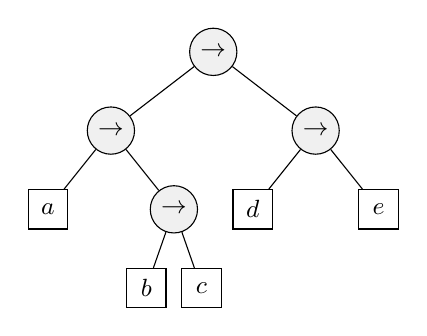
\begin{tikzpicture}[font=\small]
			\node[op] {$\rightarrow$}
				child {node[op] {$\rightarrow$}
					child {node[act] {$a$}}
					child {node[op] {$\rightarrow$}
						child {node[act] {$b$}}
						child {node[act] {$c$}}}}
				child {node[op] {$\rightarrow$}
					child {node[act] {$d$}}
					child {node[act] {$e$}}};
		\end{tikzpicture}
		\caption{Base process tree $T_{\mathit{base}}$}
		\label{fig:rheon:example_cf_tree_base}
	\end{subfigure}
	\hfill
	\begin{subfigure}{0.48\textwidth}
		\centering
		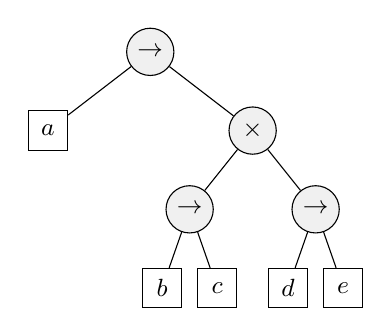
\begin{tikzpicture}[font=\small]
			\node[op] {$\rightarrow$}
				child {node[act] {$a$}}
				child {node[op] {$\times$}
					child {node[op] {$\rightarrow$}
						child {node[act] {$b$}}
						child {node[act] {$c$}}}
					child {node[op] {$\rightarrow$}
						child {node[act] {$d$}}
						child {node[act] {$e$}}}};
		\end{tikzpicture}
		\caption{Process tree $T_1$ after the drift}
		\label{fig:rheon:example_cf_tree_new}
	\end{subfigure}
	\caption[Process trees of the example log with a control-flow drift]{%
		The process trees of the example log with a sudden control-flow drift on July 1, 2020.
		\subref{fig:rheon:example_cf_tree_base}~The base process tree ${\rightarrow}({\rightarrow}(a, {\rightarrow}(b, c)), {\rightarrow}(d, e))$ produces only the trace $\seq{a, b, c, d, e}$.
		\subref{fig:rheon:example_cf_tree_new}~The process tree ${\rightarrow}(a, {\times}({\rightarrow}(b, c), {\rightarrow}(d, e)))$ produces the traces $\seq{a, b, c}$ and $\seq{a, d, e}$.}
	\label{fig:rheon:example_cf_trees}
\end{figure}

\begin{figure}[tbp]
	\centering
	\begin{subfigure}{\textwidth}
		\centering
		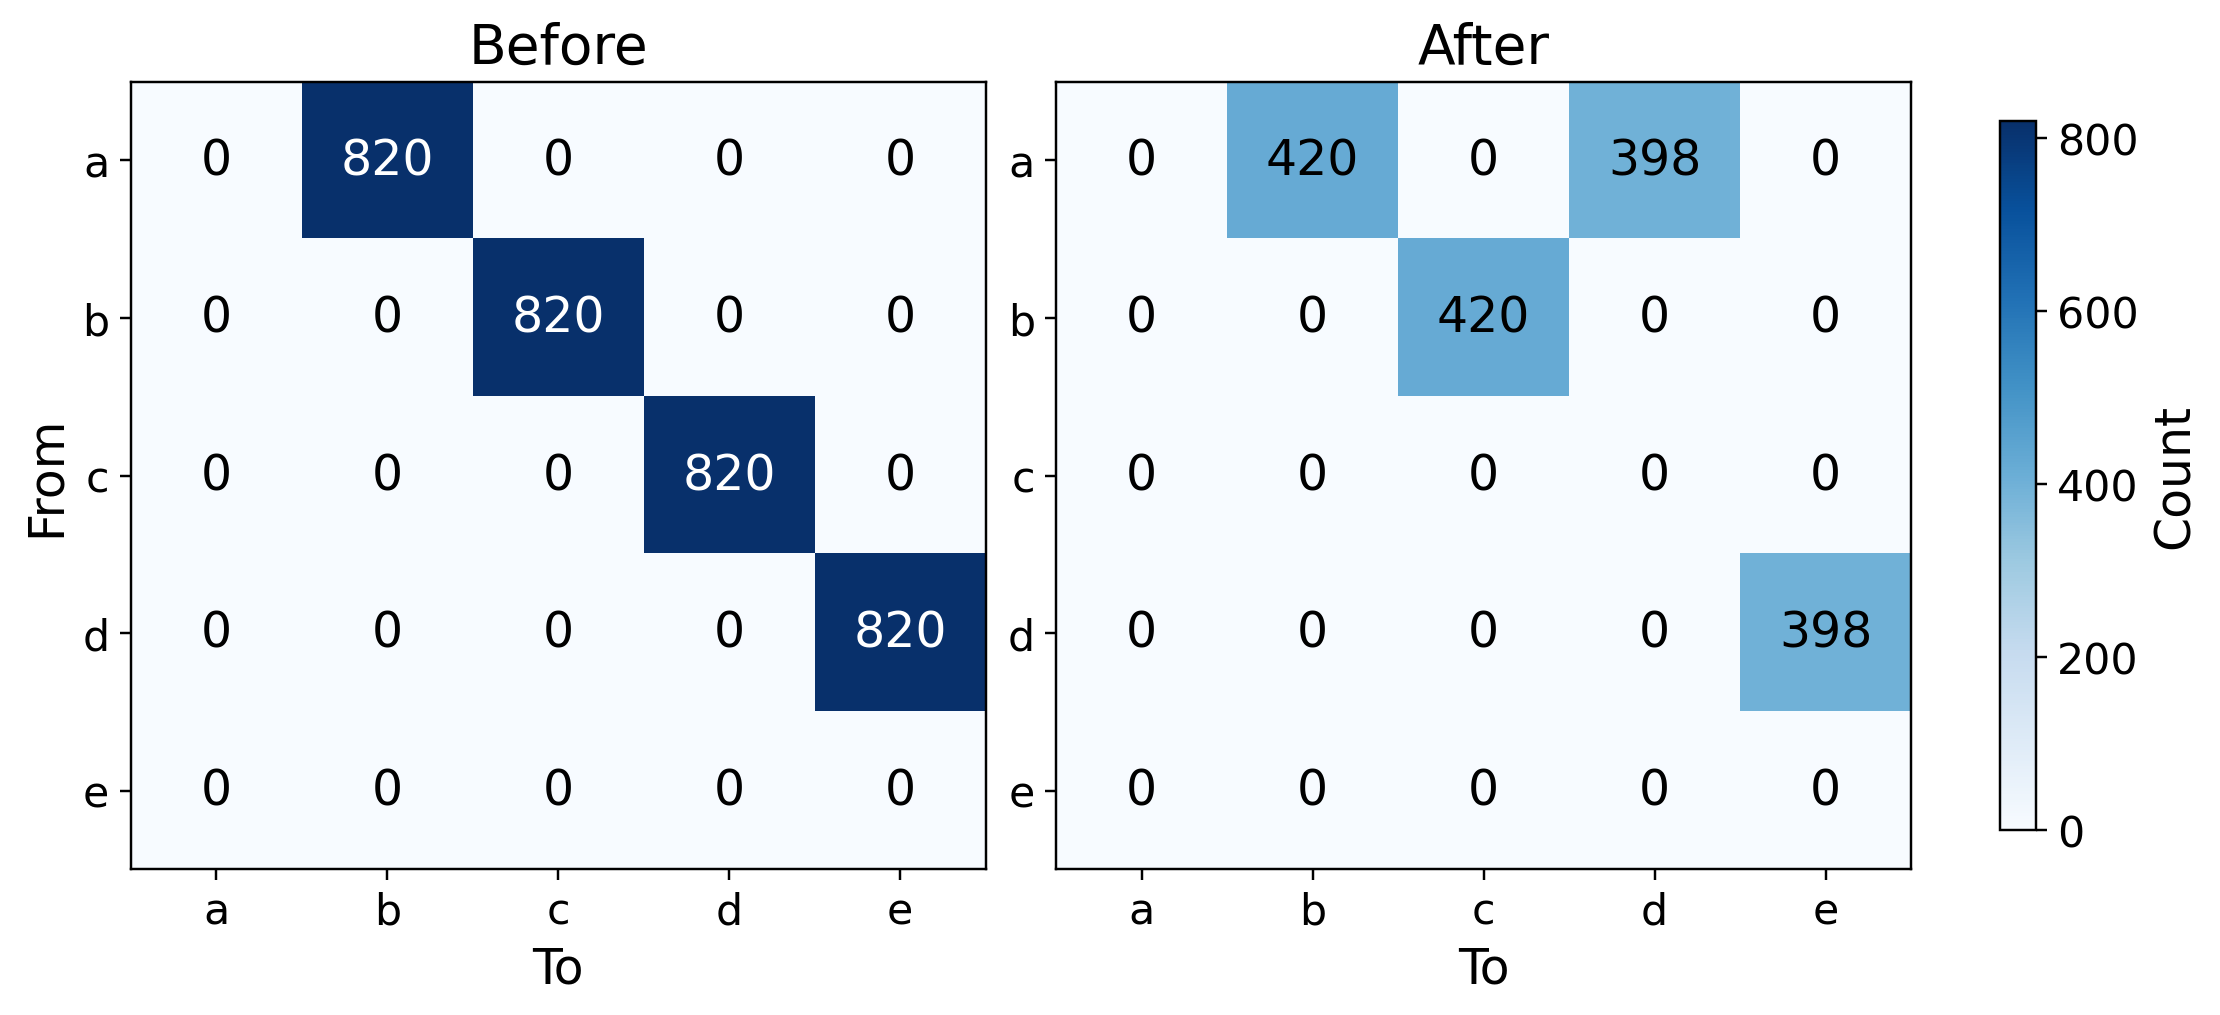
\includegraphics[width=0.85\textwidth]{figures/control_flow_counts}
		\caption{Directly-follows counts}
		\label{fig:rheon:example_cf_counts}
	\end{subfigure}

	\medskip
	\begin{subfigure}{0.3\textwidth}
		\centering
		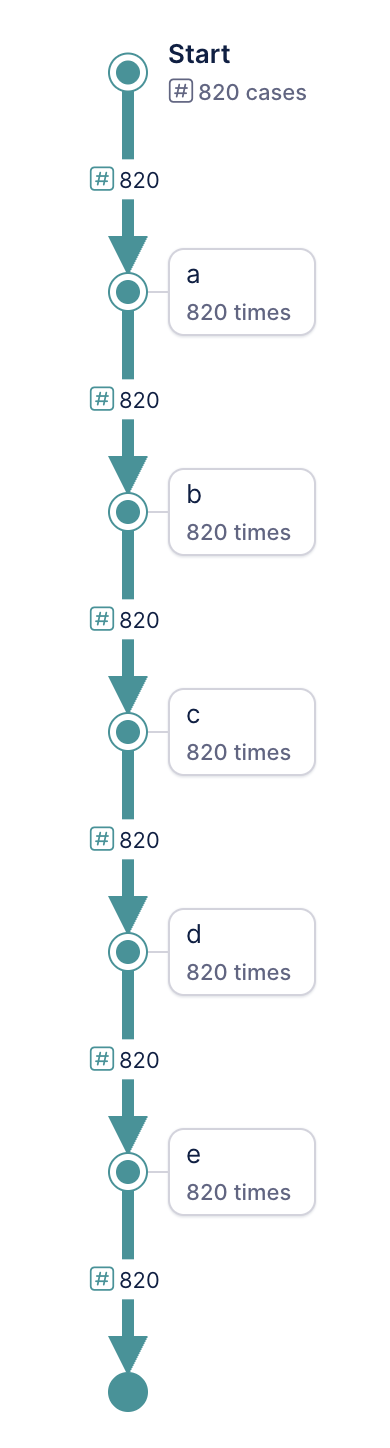
\includegraphics[height=8.6cm]{figures/celonis-variant-explorer-pre}
		\caption{Before the drift}
		\label{fig:rheon:example_cf_celonis_pre}
	\end{subfigure}
	\begin{subfigure}{0.45\textwidth}
		\centering
		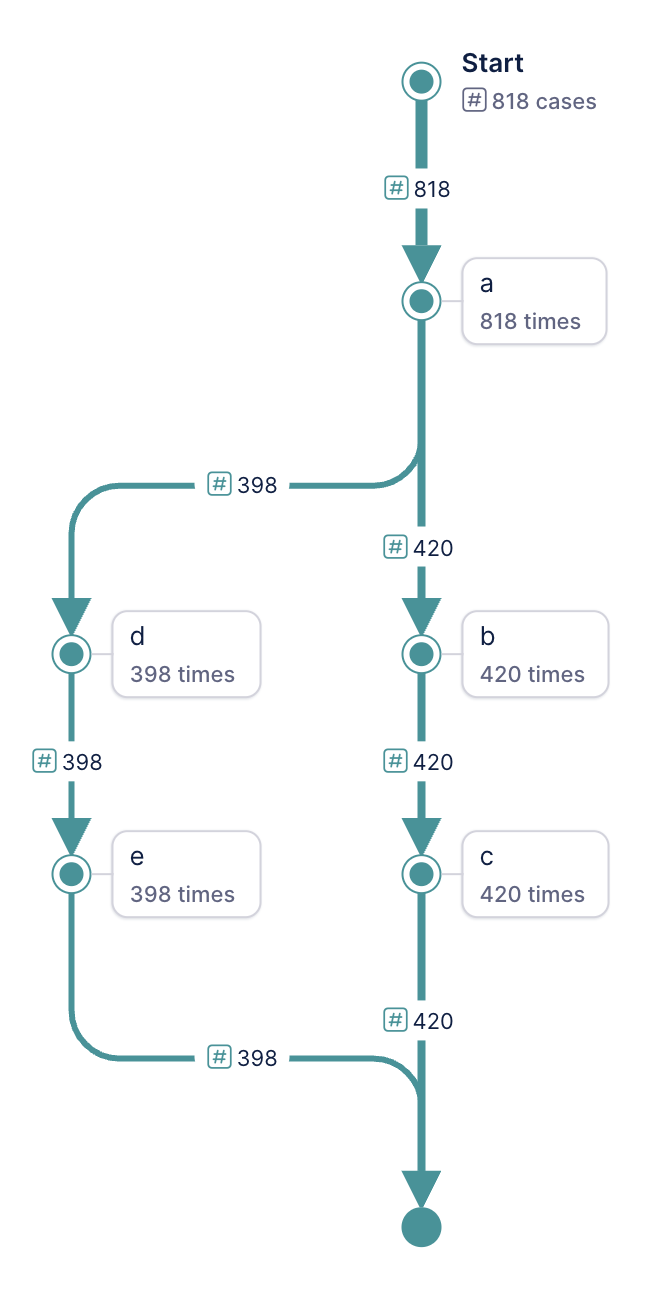
\includegraphics[height=8.6cm]{figures/celonis-variant-explorer-post}
		\caption{After the drift}
		\label{fig:rheon:example_cf_celonis_post}
	\end{subfigure}
	\caption[Example log with a control-flow drift]{%
		The example log with a sudden control-flow drift on July 1, 2020.
		\subref{fig:rheon:example_cf_counts}~Number of directly-follows relations from an activity (rows) to the next activity (columns) in the cases that arrive before (left) and after (right) the drift.
		\subref{fig:rheon:example_cf_celonis_pre} and \subref{fig:rheon:example_cf_celonis_post}~Screenshots of the variant explorer of Celonis for the cases before and after the drift. The numbers give how often each activity and each directly-follows relation occurs. Before the drift, all cases follow the trace $\seq{a, b, c, d, e}$. After the drift, a case follows either $\seq{a, b, c}$ or $\seq{a, d, e}$.}
	\label{fig:rheon:example_cf}
\end{figure}

\emph{Resource perspective:} From July 1, 2020, each activity gets a new dominant resource, e.g., activity $a$ moves from \texttt{res\_01} to \texttt{res\_02}. Figure~\ref{fig:rheon:example_res} shows how many events of each activity each resource executes before and after the drift. Before and after the drift, the dominant resource executes between 84\% and 88\% of the events of its activity. This matches the expected share of $0.8 + 0.2/3 \approx 0.87$, i.e., 87\%, for three resources.

\begin{figure}[tbp]
	\centering
	\begin{subfigure}{\textwidth}
		\centering
		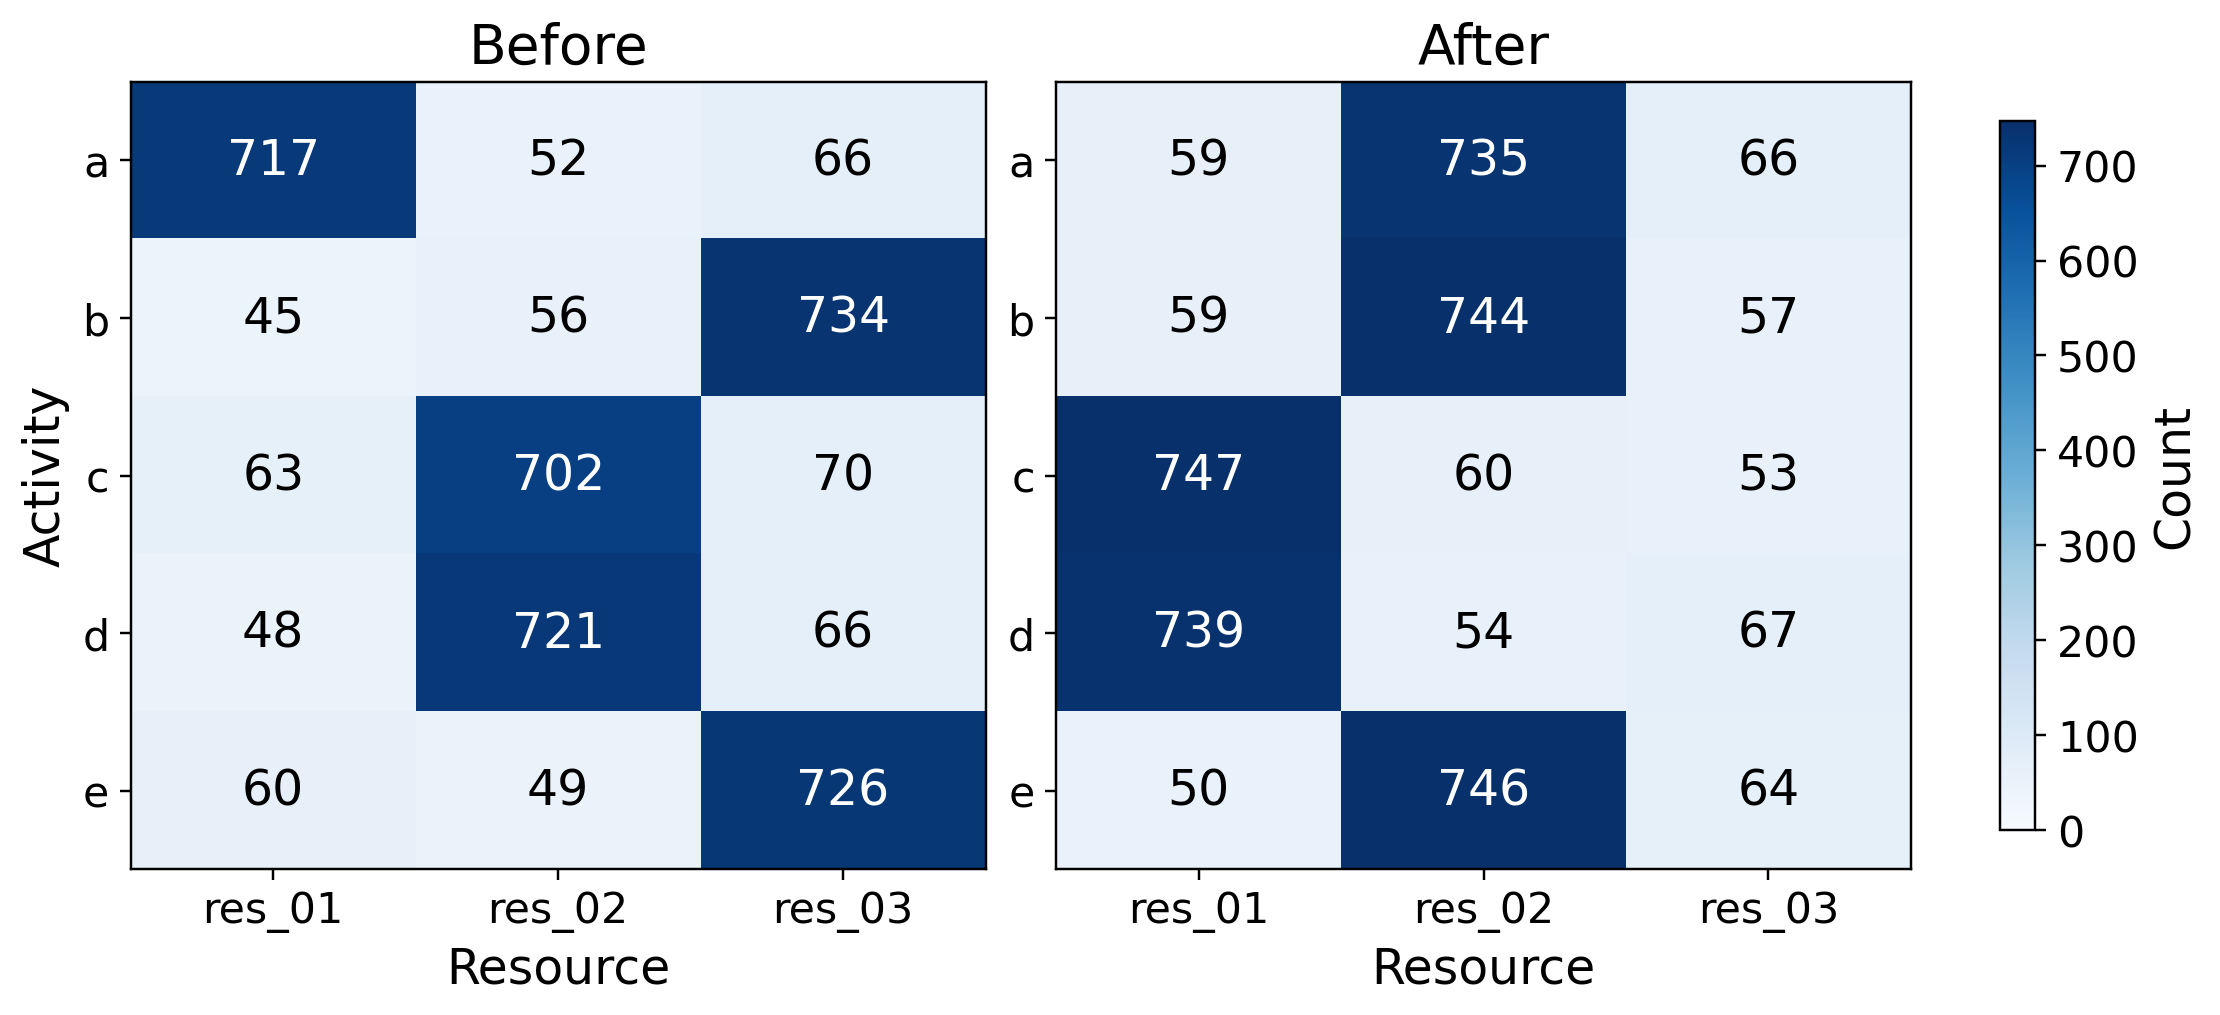
\includegraphics[width=\textwidth]{figures/resource_reassignment}
		\caption{Events per activity and resource}
		\label{fig:rheon:example_res_counts}
	\end{subfigure}

	\medskip
	\begin{subfigure}{\textwidth}
		\centering
		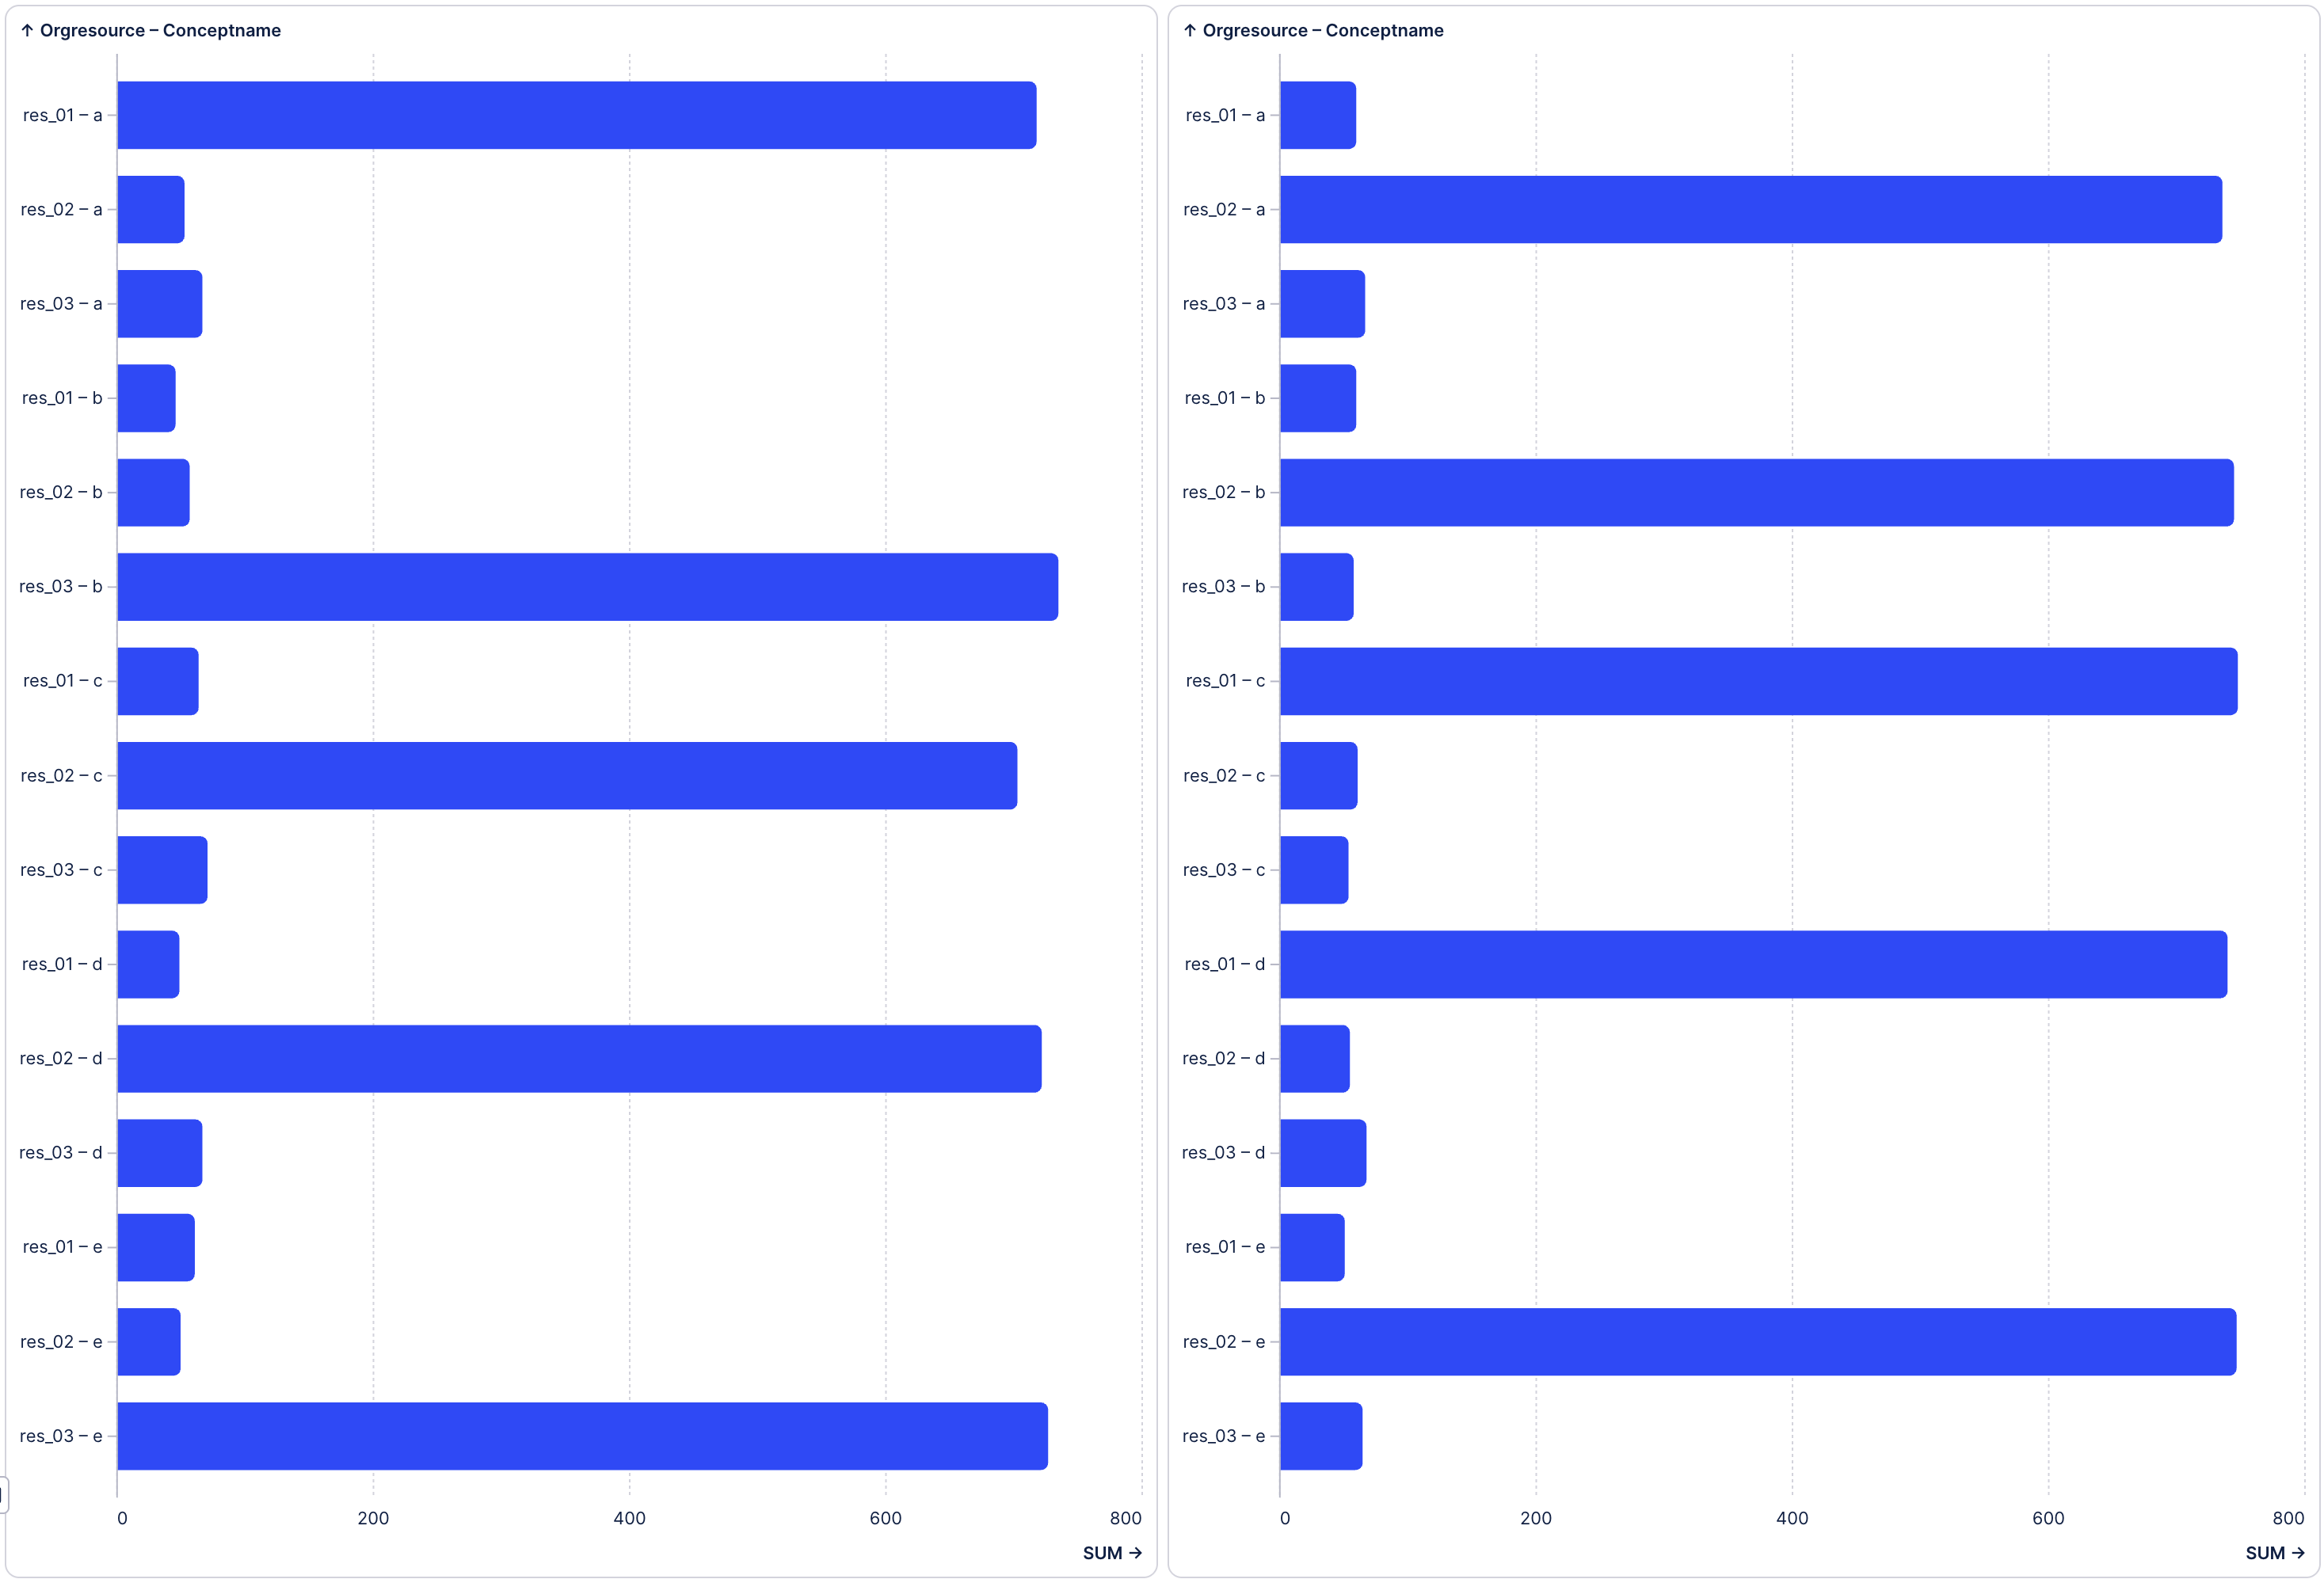
\includegraphics[width=0.9\textwidth]{figures/celonis-workload-by-activities}
		\caption{Events per resource and activity in Celonis}
		\label{fig:rheon:example_res_celonis}
	\end{subfigure}
	\caption[Example log with a reassignment drift]{%
		The example log with a sudden reassignment drift on July 1, 2020, before (left) and after (right) the drift.
		\subref{fig:rheon:example_res_counts}~Number of events of each activity (rows) that each resource (columns) executes before and after the drift.
		\subref{fig:rheon:example_res_celonis}~Screenshot of Celonis with the same numbers as bars for each pair of resource and activity. After the drift, each activity has a new dominant resource, e.g., $a$ moves from \texttt{res\_01} to \texttt{res\_02}.}
	\label{fig:rheon:example_res}
\end{figure}

\emph{Inter-case perspective:} From July 1, 2020, the mean inter-arrival time rises from 219 to 4,380 minutes, so cases arrive 20 times less often. Thus, 1,214 cases arrive before the drift and only 74 cases after it. All cases follow the same trace $\seq{a, b, c, d, e}$. Figure~\ref{fig:rheon:example_inter} shows the events of the cases over time in the dotted chart of Celonis. Before the drift, the cases form a steep line, and after the drift, only a few cases arrive.

\begin{figure}[tbp]
	\centering
	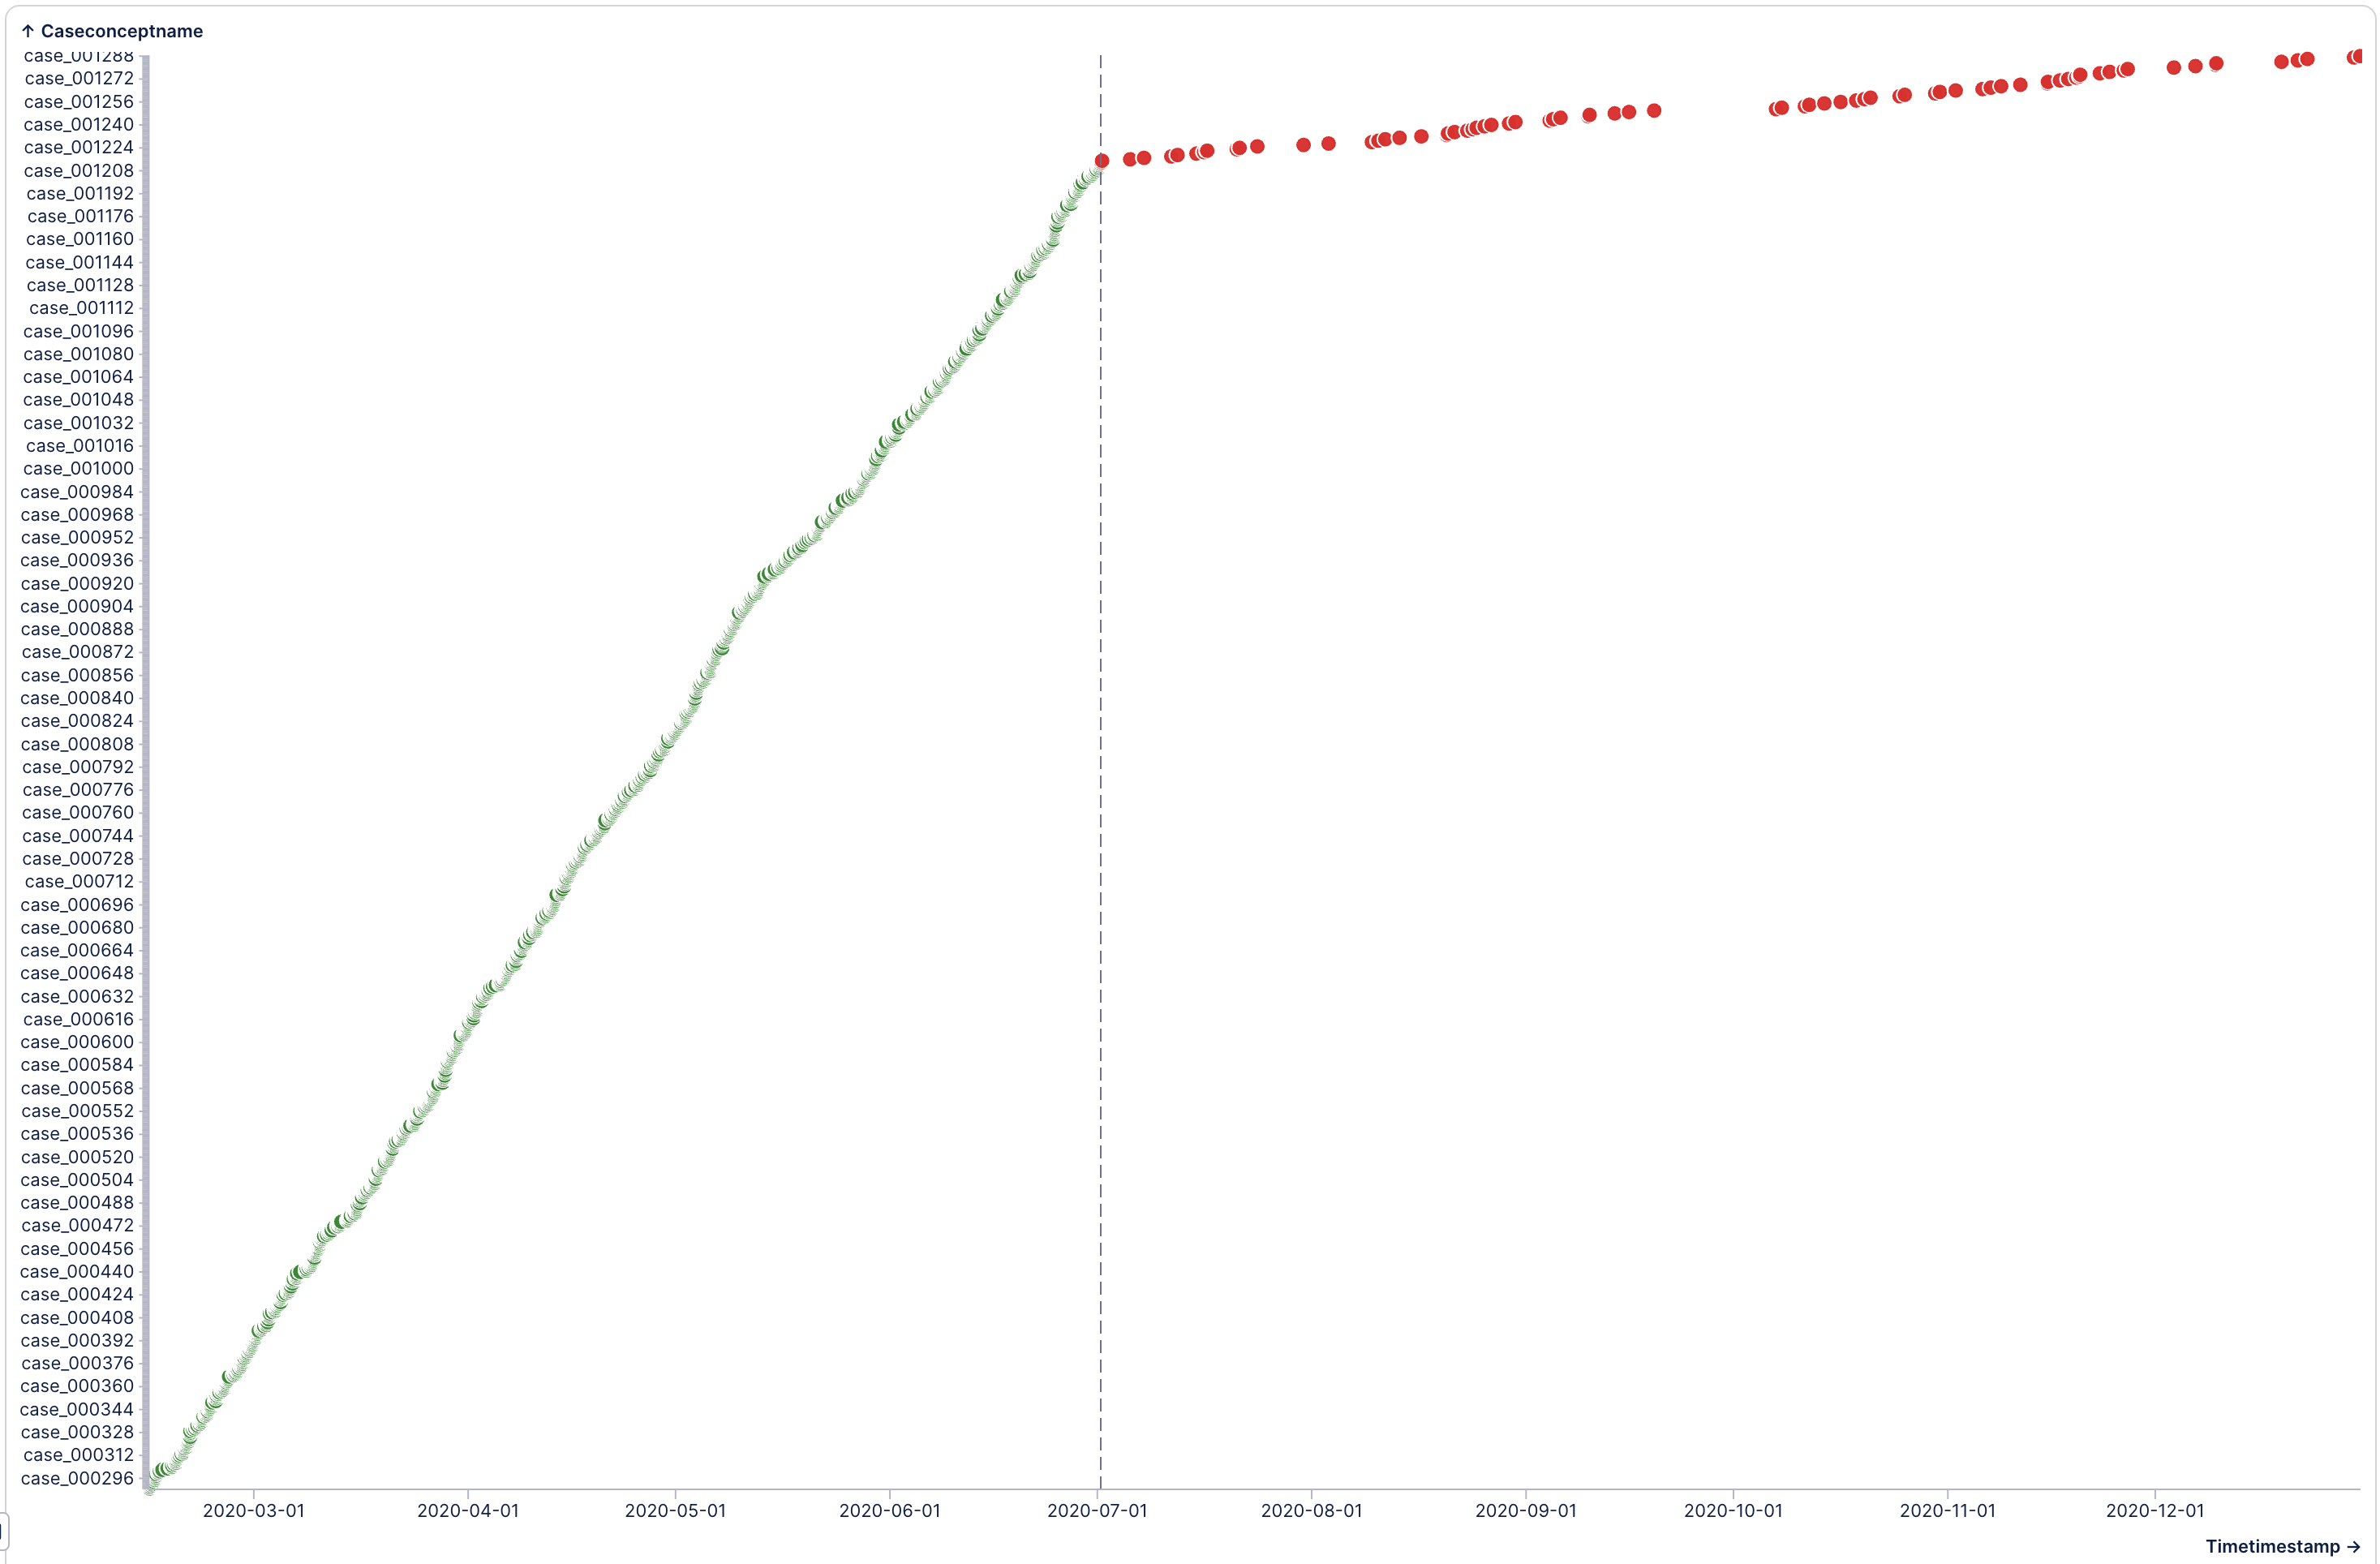
\includegraphics[width=\textwidth]{figures/celonis-dotted-chart-by-drift}
	\caption[Example log with an arrival rate drift]{%
		Screenshot of the dotted chart of Celonis for the example log with a sudden arrival rate drift on July 1, 2020 (dashed line). Each dot is an event, placed at its time and at its case, with the cases ordered by their arrival. The chart shows the cases from February 2020 on, with the cases before the drift in green and after the drift in red. After the drift, the mean inter-arrival time rises from 219 to 4,380 minutes, so only a few cases arrive.}
	\label{fig:rheon:example_inter}
\end{figure}

\section{Limitations and Future Work}
\label{sec:rheon:limitations}
Rheon is a prototype that we develop continuously, so it can still contain bugs. Rheon does not simulate a full operational process. It generates the behavior from process trees and adds times, resources and case attributes to the cases, but it does not model, e.g., the capacities of resources. The generated logs are therefore controlled test data and not replicas of real processes. Compared to CDLG, which also generates incremental and recurring drifts as well as noisy traces~\autocite{grimm2022cdlg}, Rheon currently supports only sudden and gradual drifts without noise. Future work could extend Rheon with further drift types and drift modes. We also plan to generate object-centric event logs, from which \textcite{berti2025ocel} compute execution states.
